%% Copyright (c) 2022 Martín E. Zahnd
%%
%% This code is licensed under MIT license (see LICENSE.txt for details)
%%
\chapter{Repaso de Álgebra}
\graphicspath{ {./teoria/resources/repaso/} }

Una aclaración importante previo a comenzar es que en este apunte vamos a 
considerar $0 \in \mathbb{N}$.

\section{Producto cartesiano}

\begin{definicion}{Producto cartesiano}{}
    \begin{enumerate}
    
        \item Sean $A_1$ y $A_2$ conjuntos.
    
        \begin{gather*}
            A_1 \times A_2 = \{ (x,y) / x \in A_1, y \in A_2 \} 
        \end{gather*}
    
        \bigskip
        \textbf{Notación:} $A_1 = A_2 = A \implies A \times A = A^2$
    
        \item Sean $A_1, \dotsc, A_n$ conjuntos.
    
        \begin{gather*}
            A_1 \times \dots \times A_n 
                = \{ (x_1, \dotsc, x_n) / x_i \in A_i, 1 \leq i \leq n \}
        \end{gather*}
    
        \bigskip
        \textbf{Notación:} 
        $A_1 = \dots = A_n = A \implies A \times \dots \times A = A^n$
    
    \end{enumerate}
\end{definicion}

\section{Relaciones}

\begin{definicion}{Relaciones}{}
    \begin{enumerate}
        \item Sea $A$ un conjunto, una relación unaria en $A$ es cualquier 
            subconjunto $\mathcal{R} \subseteq A$.
    
        
        \item Sean $A_1 , \dotsc , A_n$ conjuntos. Una relación n-aria es un 
            subconjunto $\mathcal{R}\subseteq A_1 \times \dots \times A_n$.
    
    \end{enumerate}
\end{definicion}

Notemos que una relación 1-aria definida en $A$ es cualquier 
subconjunto $\mathcal{R} \subseteq A$. Mientras que una relación en
la que $n=2$ se denomina ``binaria''.

Si $A_1 = \dots = A_n = A$, se dice que la relación n-aria está 
definida en $A$.

\subsubsection{Ejemplos}

\begin{enumerate}
    \item
    \begin{gather*}
        A = \{ x/x \text{ es alumno del ITBA} \} \\
        R = \{ x \in A / x \text{ es alumno de lógica} \}
    \end{gather*}

    \item $A = \mathbb{R}$. Sea $\mathcal{R} \subseteq \mathbb{R}^3$

        \[ \mathcal{R} = 
        \{ (x,y,z) \in \mathbb{R}^3 / x^2 + y^2 + z^2 = 1 \} \]

    \item $A = \{ \text{alumnos del ITBA} \}$

        \[ \mathcal{R} 
        = \{ (x,y) \in A^2 / x \text{ cursa alguna materia con y}\} \]
\end{enumerate}

\subsection{Clasificación de relaciones binarias}

Sea $\mathcal{R} \subseteq A \times A$

\bigskip
\textbf{Notación:} $(x,y) \in \mathcal{R} \iff x \mathcal{R} y$

\begin{enumerate}
    \item[\circled{R}] $\mathcal{R}$ es reflexiva si $\forall x \in A$, $x \mathcal{R} x$
    \item[\circled{S}] $\mathcal{R}$ es simétrica si $\forall x,y \in A$, 
        $x \mathcal{R} y \implies y \mathcal{R} x$
    \item[\circled{T}] $\mathcal{R}$ es transitiva si $\forall x, y, z \in A$,
        $x \mathcal{R} y \wedge y \mathcal{R} z \implies x \mathcal{R} z$
    \item[\circled{A}] $\mathcal{R}$ es antisimétrica si $\forall x, y \in A$,
        $x \mathcal{R} y \wedge y \mathcal{R} x \implies x = y$
    \item[\circled{E}] $\mathcal{R}$ es de equivalencia si es reflexiva, simétrica y 
        transitva.
    \item[\circled{O}] $\mathcal{R}$ es de orden (parcial) si es reflexiva, transitiva y
        antisimétrica.
    \item[\circled{OT}] $\mathcal{R}$ es de orden total si es de orden parcial y
        $\forall x, y \in A$, $x \mathcal{R} y \vee y \mathcal{R} x$
\end{enumerate}

\subsection{Partición}

Sea $A \neq \varnothing$. Una partición de $A$ es una familia de conjuntos
$\mathcal{F} = \{ A_i \}_{i \in I}$ tal que:

\begin{enumerate}
    \item $A_i \neq \varnothing$ \nota{$\forall i \in I$}%
    \item $A_i \subseteq A$ \nota{$\forall i \in I$}%
    \item $A_i \cap A_j = \varnothing$ \nota{$i \neq j$, $\; \forall i,j \in I$}%
    \item $\bigcup_{i \in I} A_i = A$
\end{enumerate}

\subsubsection{Ejemplos}

Sean $A = \mathbb{N}$, $A_1 = \{ x \in \mathbb{N} / x \text{ es par} \}$,
$A_2 = \{ x \in \mathbb{N} / x \text{ es impar} \}$.

\begin{gather*}
    \mathcal{F} = \{ A_1, A_2 \} \text{ es una partición en } \mathbb{N} 
\end{gather*}


\begin{figure}[H]
    \centering
    \includegraphics[width=0.20\textwidth]{particion_n_pares_impares}
    \caption{Partición de $\mathbb{N}$ en pares e impares.}
\end{figure}

\subsection{Propiedades}

\begin{enumerate}
    \item $\mathcal{R}$ es de equivalencia en $A \implies \mathcal{R}$ induce
        una partición en $A$.
    \item $\mathcal{F}$ es una partición de $A \implies \mathcal{F}$ induce
        una relación de equivalencia en $A$.
\end{enumerate}

\section{Conjunto cociente}
\begin{definicion}{Conjunto cociente}{}
    Sea $\mathcal{R}$ una relación de equivalencia en $A$, se define el conjunto
    cociente como:

    \begin{gather*}
        \nicefrac{A}{R} = \{ \overline{x} / x \in A \}
        \notamath{$\overline{x}$ es la partición de $A$ inducida por $\mathcal{R}$}
    \end{gather*}
\end{definicion}

\medskip

Recordemos la definición de clase de equivalencia. 

\begin{definicion}{Clase de equivalencia}{}
    Sea $x \in A$.
    \begin{gather*}
        \overline{x} = \{ y \in A / x \mathcal{R} y \}
    \end{gather*}
\end{definicion}

\subsubsection{Ejemplos}

\begin{enumerate}
    \item $\mathcal{R} = \{ (x,y) \in \mathbb{Z}^2 / 
        \underbrace{\divides{2}{x-y}}_{x \equiv y (2)} \}$ 

        En este caso hay solamente dos clases en la relación de congruencia
        módulo dos: la clase donde están todos los números pares, y en la que
        están todos los impares.

        \[ \nicefrac{\mathbb{Z}}{\mathcal{R}} 
            = \{ \overline{0}, \overline{1} \} 
        = \mathbb{Z}_2 \]

    \item $\mathcal{R} = \{ (x,y) \in \mathbb{Z}^2 / x \equiv y (n) \}$

        \[ \nicefrac{\mathbb{Z}}{\mathcal{R}} 
        = \{\overline{0}, \overline{1}, \dotsc, \overline{n-1} \} 
        = \underbrace{\mathbb{Z}_n}_{\text{Son anillos}} \]

        En $\mathbb{Z}_3$, por ejemplo, tendríamos 
        $\mathcal{R}=\{ (x,y)\in \mathbb{Z}^2 / x \equiv y(3) \}$

        \begin{gather*}
            \nicefrac{\mathbb{Z}}{\mathcal{R}} = \{ \overline{0},
            \overline{1},\overline{2} \} = \mathbb{Z}_3
        \end{gather*}
        
        En $\mathbb{Z}_5$, 
        \[\underbrace{\overline{2}}_{\equiv \overline{7}} 
        + \underbrace{\overline{4}}_{\equiv \overline{-1}} 
        = \overline{6} = \overline{1} \]

        Notemos que por la congruencia, obtenemos el mismo resultado:
        \[ \overline{7} + \overline{(-1)} = \overline{6} = \overline{1} \]

        \bigskip
        \textit{Observación:} 
        \nota{``Buena definición'' de la suma en $\mathbb{Z}_n$}%
        Recordemos esta propiedad de congruencia:

        Sean $a \equiv b(n)$ y $c \equiv d (n)$, entonces $a+c \equiv b+d(n)$

    \item $\mathcal{R} = \{z,w \in \mathbb{C}^2 / |z| = |w| \}$

        \[ \nicefrac{\mathbb{C}}{\mathcal{R}} = \mathbb{R}_{\geq 0}\]

        \begin{figure}[H]
            \centering
            \includegraphics[width=0.35\textwidth]{clase_de_z_complejo.png}
            \caption{Clases de $z$, con $z \in \mathbb{C}$.}
        \end{figure}

    \item Sean $X = \{ a,b,c,d\}$ y 
        $\mathcal{R} = \{ (a,b), (b,b), (c,c), (d,d), (a,b), (b,a) \}$
        
        \nota{Notemos que $\overline{a}$ cubre el par $(a,a)$ y $(b,b)$
        pues $a$ y $b$ se relacionan: $(a,b)$ y $(b,a)$}%
        \[ \nicefrac{X}{\mathcal{R}} = \{ \overline{a}, \overline{c},
        \overline{d} \}\]

        \item ¿Cuántas relaciones de equivalencia se pueden definir en 
            $A = \{1,2,3\}$?

        Contamos las particiones: 

        Si la partición tiene 3 conjuntos, entonces hay una única partición; 
        si hay un único conjunto, es un caso trivial y tendremos también una
        única partición. 

        El caso restante es tener dos conjuntos, en esta situación un conjunto 
        tendrá un único elemento y otro va a tener dos, con lo cual tendremos 
        $\binom{3}{1} = 3$ particiones.

        Por lo tanto, se pueden definir 5 relaciones de equivalencia.
\end{enumerate}



\section{Operaciones en anillos}

Tenemos las siguientes operaciones definidas en $Z_n$:

\begin{itemize}
    \item $\overline{a} + \overline{b} = \overline{a+b}$
    \item $\overline{a} \cdot \overline{b} = \overline{a \cdot b}$
\end{itemize}

\section{Funciones}

\begin{definicion}{Función}{}
    Sean $A$ y $B$ conjuntos.

    Una función de $A$ en $B$ \nota{$f: A \to B$} es una relación $\mathcal{R}
    \subseteq A \times B$ que verifica:

    \begin{gather*}
        \forall x \in A,
        ~ \exists ! \, y \in B
        / (x,y) \in \mathcal{R} \notamath{$A$: Dominio\\ $B$: Codominio}
    \end{gather*}

    \bigskip
    \textbf{Notación:} $y = f(x)$
\end{definicion}

\subsubsection{Ejemplos}
\begin{enumerate}
    \item $\mathcal{R} = \{(x,y) \in \mathbb{R}^2 / y = x\}$ es una función 
        $f: \mathbb{R} \to \mathbb{R}, f(x) = x$. 
        \nota{Esta es la función identidad}%

    \item $\mathcal{R} = \{ (x,y) \in \mathbb{Z}^2 / \divides{x}{y} \}$ no es
        función pues no hay una única imagen:

        \begin{center}
          \begin{tabular}{c c c}
              $(2,4) \in \mathbb{R}$ & $(2,8) \in \mathbb{R}$ & pero $4 \neq 8$
          \end{tabular}
        \end{center}
    \item $\mathcal{R} = \{ (x,y) \in \mathbb{R} \times \mathbb{N} / x = y\}$
        no es función pues: 
        \begin{gather*}
            \sqrt{2} \notin Dom(\mathcal{R})
        \end{gather*}

    \item $\mathcal{R} = \{(x,y,z) \in 
        \underbrace{\mathbb{R}^3}_{\mathbb{R}^2 \times \mathbb{R}} / 
        x^2 + y^2 + z = 0\}$ es función.
        
        \begin{gather*}
            f: \mathbb{R}^2 \to \mathbb{R}, \; f(x,y) = -x^2 - y^2
        \end{gather*}

    \item $\mathcal{R} = \{ (x,y,z) \in \mathbb{R}^3 / x^2 + y^2 + z^2 = 1 \}$
        no es función.

        \begin{center}
            \begin{tabular}{c c c}
                $(0,0,1) \in \mathbb{R}$ & $(0,0,-1) \in \mathbb{R}$ & 
                pero $1 \neq -1$
            \end{tabular}
        \end{center}
\end{enumerate}

\bigskip
\textit{Observación:} 
Sean $A_1, \dotsc, A_n$ conjuntos, 
$\mathcal{R} \subseteq A_1 \times \dots \times A_n$ relación n-aria.

Se puede pensar a $\mathcal{R}$ como una relación binaria: 
$\mathcal{R} \subseteq A \times B$ donde $A = A_1 \times \dots A_{n-1}$ y 
$B = A_n$.

Diremos que $\mathcal{R}$ es una función de $n-1$ variables si 
$\mathcal{R} \subseteq A \times B$, $A$ es el producto cartesiano de $n-1$ 
conjuntos y $\mathcal{R}$ es función.

Es decir, 
    \begin{center}
        $\forall x \in A \; \exists ! \, y \in B / (x,y) \in \mathcal{R}$

        $\iff$

        $\forall (x_1, \dotsc, x_{n-1}) \in A = A_1 \times \dots \times A_{n-1}
        \; \exists ! \, y=x_n \in A_n = B / (x_1, \dotsc, x_n) \in \mathcal{R}$
    \end{center}


\subsection{Clasificación de funciones}

Sea $f: A \to B$ una función.

\begin{itemize}
    \item $f$ es inyectiva si $f(x) = f(y) \implies x = y$
    \item $f$ es sobreyectiva si $\forall y \in B$  $\exists \, x \in A / f(x)=y$
        \nota{Es decir, $Im(f) = B$}%
    \item $f$ es biyectiva si es inyectiva y sobreyectiva.
\end{itemize}

\subsubsection{Ejemplos}

\begin{enumerate}
    \item $f: \mathbb{R} \to \mathbb{R} / f(x) = x^3$
        \begin{itemize}
            \item Inyectiva:

                \begin{gather*}
                    f(x) = f(y) \implies x^3 = y^3 \implies \sqrt[3]{x^3}
                    = \sqrt[3]{y^3} \implies x = y
                \end{gather*}

            \item Sobreyectiva:
                Sea $y \in \mathbb{R}$, busco $x \in \mathbb{R} /f(x)=y$.

                Tomo $x = \sqrt[3]{y}$

                \begin{gather*}
                    \implies f(x) = {\left(\sqrt[3]{y} \right)}^3 = y
                \end{gather*}

            \item Biyectiva: Como $f$ es inyectiva y sobreyectiva, entonces 
                $f$ es biyectiva.
        \end{itemize}

    \item $f: \mathbb{C} \to \mathbb{C} / f(z) = z^3$

        \begin{itemize}
            \item Inyectiva: No es inyectiva.

                Supongamos que $z \in \mathbb{C} / z^3 = 1 \iff z^3-1 = 0$.
                Notemos que esto es un polinomio de grado 3, y, por el teorema
                fundamental del álgebra (TFA), existen 3 raíces del polinomio
                $x^3-1$ en $\mathbb{C}$
                \nota{$(x-1)^3 \neq x^3 -1$}%

                Como hay al menos 2 raíces distintas, entonces existen $z_1$,
                $z_2$, tal que $f(z_1) = f(z_2) = 1 \implies$ no es inyectiva.

                Otra forma es notar que $f(1) = 1$ y también 
                
                \[ f \left(\cos{\left(\frac{2}{3} \pi \right)} 
                    + i \sin{\left(\frac{2}{3} \pi\right)}\right) =
                \cos{\left(3 \; . \; \frac{2}{3} \pi\right)} 
            + i \sin{\left(3 \; . \; \frac{2}{3} \pi\right)} = 1 \]

            \item Sobreyectiva: Tarea.

            \item Biyectiva: Como no es inyectiva, tampoco es biyectiva. 
        \end{itemize}
\end{enumerate}


\subsection{Extensión y restricción de funciones}

\begin{definicion}{Extensión de una función}{}
    Sea $f: A \to B$ una función. 

    Sea $C$ un conjunto tal que $A \subseteq C$ y $D$ un conjunto tal que 
    $D \subseteq B$.

    \medskip
    
    \nota{Defino la función $\tilde{f}$ en un conjunto más grande que $f$, pero 
    ambas coinciden sobre $A$.}%
    Entonces la función $\tilde{f}: C \to D$ es una extensión de $f$ si 
    $\frest{\tilde{f}}{A} = f$, es decir, 
    $\tilde{f}(a) = f(a)$, $\forall a \in A$

\end{definicion}

\bigskip
La restricción de $f$ a $A$ queda entonces definida como:

\begin{definicion}{Restricción de una función}{}
    Sea $f: A \to B$ una función. 

    \medskip

    \begin{center}
        $\frest{\tilde{f}}{A}: A \to B$ es una función tal que 
        $\frest{\tilde{f}}{A} (x) = f(x)$, $\forall x \in A$
    \end{center}
\end{definicion}

\subsubsection{Ejemplos}

\begin{enumerate}
    \item Hallar extensiones a $\mathbb{R}$ de $f: \mathbb{R}_{\geq 0} \to 
        \mathbb{R} / f(x) = x$
        \nota{Pedir una ``extensión a $\mathbb{R}$'' es pedir que el dominio
        de la función extendida sea $\mathbb{R}$.}%

        \begin{enumerate}
            \item $\tilde{f}_1 : \mathbb{R} \to \mathbb{R} / \tilde{f}_1(x)=x$
            \item $\tilde{f}_2 : \mathbb{R}\to\mathbb{R} / \tilde{f}_2(x)=|x|$

                También es una extensión porque si nos restringimos a los 
                $x \geq 0$, tenemos que $|x| = \underbrace{x}_{f(x)}$

            \item $\tilde{f}_3: \mathbb{R}\to\mathbb{R}/\tilde{f}_3(x)=
                \begin{cases}
                    \overbrace{x}^{f(x)} & \text{si } x \geq 0 \\
                    2 & \text{si } x<0
                \end{cases}$

        \end{enumerate}
    Notar que hay infinitas extensiones con distintas propiedades.
    
    Por ejemplo, $\tilde{f}_1$ es continua y derivable, $\tilde{f}_2$
    es continua y no derivable, y $\tilde{f}_3$ no es continua.

    \item Hallar extensiones a $\mathbb{R}$ de $f: \mathbb{R}-\{0\} \to
        \mathbb{R} / f(x) = \frac{\sin{(x)}}{x}$. ¿Existe alguna extensión
        continua?

        \begin{enumerate}
            \item $\tilde{f}_1: \mathbb{R}\to\mathbb{R} / \tilde{f}_1 (x) =
                \begin{cases}
                    \frac{\sin{(x)}}{x} & x \neq 0 \\
                    7 & x = 0
                \end{cases}$

            \item Supongamos que $\tilde{f}$ es una extensión continua. 
                \begin{align*}
                    \implies &\underbrace{\lim_{x\to 0} f(x)} = \tilde{f}(0)\\
                             &\lim_{x\to 0} f(x) = 1
                \end{align*}

                Entonces existe una única extensión continua:
                \[\tilde{f}(x) = \begin{cases}
                    \frac{\sin{(x)}}{x} & x \neq 0 \\
                    1 & x = 0
                \end{cases}\]
        \end{enumerate}

    \item Hallar extensiones a $\mathbb{R}$ de $f: \mathbb{R}-\{0\} \to
        \mathbb{R} / f(x) = \frac{1}{x}$. ¿Existe alguna extensión continua?

        \begin{gather*}
            \notamath{Para algún $a\in\mathbb{R}$}
            \tilde{f}: \mathbb{R}\to\mathbb{R} / f(x) = 
            \begin{cases}
                \frac{1}{x} & x \neq 0\\
                a & x = 0 
            \end{cases}
        \end{gather*}

        Si existe una extensión continua $\tilde{f}$,
        \begin{align*}
            \implies &\underbrace{\lim_{x \to 0} \; f(x)} = \tilde{f}(0)\\
                = & \lim_{x\to 0} \; \frac{1}{x} = \infty 
        \end{align*}

        \begin{gather*}
            \therefore \; \nexists \text{ extensión continua}
        \end{gather*}
\end{enumerate}

\section{Números complejos}

Recordemos que un número complejo $z \in \mathbb{C}: z = a + i b$ puede ser
escrito de la siguiente manera:
\begin{gather*}
    z = e^{i\beta} = \cos{(\beta)} + i \sin{(\beta)}
\end{gather*}

\subsection{Conjunto Gn}

\begin{definicion}{Conjunto $G_n$}{}

    \begin{gather*}
        G_n = \{ z \in \mathbb{C} / z^n = 1 \} 
        = \{ z=e^{i\frac{2k\pi}{n}}, \; k = 0, \dotsc, n-1 \}
    \end{gather*}

\end{definicion}



\section{Transformaciones lineales}

\begin{definicion}{Transformación lineal}{}
    Sean $V$ y $W$ espacios vectoriales.

    \medskip

    Se dice que $T: V \to W$ es una transformación lineal (T.L.) si:

    \begin{enumerate}
        \item $T(u+v) = T(u) +T(v), \quad \forall u,v \in V$ 
        \item $T(\alpha u) = \alpha T(u), \quad \forall u \in V, 
            \forall \alpha \in K$
    \end{enumerate}
\end{definicion}


\subsubsection{Ejemplo}

\begin{itemize}
    \item Sea $T: \mathbb{R}^2 \to \mathbb{R} / T(x,y) = 3x-2y$. Verificar si
        $T$ es una transformación lineal.

        \begin{enumerate}
            \item Sean $u = (x_1, y_1)$ y $v = (x_2, y_2)$.

                \begin{align*}
                    T(u+v) = T(x_1 + x_2, y_1 + y_2) &= \\
                    &= 3(x_1 + x_2) - 2 (y_1 + y_2) \\
                    &= 3 x_1 - 2 y_1 + 3x_2 - 2 y_2 \\
                    &= T(x_1, y_1) + T(x_2, y_2) \\
                    &= T(u) + T(v)
                \end{align*}

            \item Sea $\alpha \in \mathbb{R}$
                \begin{align*}
                    T(\alpha u) = T(\alpha x_1, \alpha y_2) &= \\
                    &= 3 \alpha x_1 - 2 \alpha y_2 \\
                    &= \alpha (3x_1 - 2y_1) \\
                    &= \alpha T(u)
                \end{align*}
        \end{enumerate}

        Por lo tanto, $T$ es una T.L.

    \item Sea $T: \mathbb{R}^2 \to \mathbb{R}^3 / T(x,y) = (x^2,1,2y)$.
        Decidir si $T$ es una T.L.

        Tomemos $u = (1,2)$ y $v=(0,5)$.

        \begin{enumerate}
            \item $T(u+v) = T(1,7) = (1,1,14)$
            \item $T(u)+ T(v) = T(1,2) + T(0,5) = (1,1,4)+(0,1,10)=(1,2,14)$
        \end{enumerate}

        Por lo tanto, $T$ no es T.L.
\end{itemize}


\begin{teorema}{}{base-tl}
    Sean $v, w$ un $K\mathrm{-}ev$. 

    Sea $B=\{ v_1, \dotsc, v_n \}$ una base
    de $V$ y $\{ w_1, \dotsc, w_n \} \subseteq W$.

    \medskip

    Entonces existe una única transformación lineal de la forma:
    \begin{gather*}
        T \, . \, V \to W / T(v_i) = w_i
        \notamath{$i = 1, \dotsc, n$}
    \end{gather*}
    
\end{teorema}

\subsubsection{Ejemplo}

Consideremos $V = W = \mathbb{R}^2$.

Hallar $\tilde{f} : V \to W$ que extienda a $f$ dada por:
\begin{itemize}
    \item $f(1,0)=(4,-1)$
    \item $f(1,1)=(0,4)$
\end{itemize}


Propongo
\begin{gather*}
    \tilde{f}(x,y) = 
    \begin{cases}
         (4,-1) & \text{si }(x,y)=(1,0) \\
         (0,4) & \text{si } (x,y) = (1,1) \\
         (0,0) & \text{en otro caso}
    \end{cases}
\end{gather*}

\textit{¿Existe alguna extensión que sea T.L.?}

La respuesta es que sí, por el Teorema \ref{teo:base-tl}.

Como $B=\{ (1,0); (1,1) \}$ es base de $\mathbb{R}^2$

\begin{gather*}
    \implies \forall (x,y) \in \mathbb{R}^2, \exists ! \; \alpha, \beta
    \in \mathbb{R} / (x,y) = \alpha(1,0) + \beta (1,1)
\end{gather*}

Encontremos $\alpha$ y $\beta$.

\begin{gather*}
    \begin{cases}
        x = \alpha + \beta \implies \alpha = x -\beta\implies
        \dashbox{$\alpha = x - y$} \\
        \dashbox{$y = \beta$}
    \end{cases}
\end{gather*}

Entonces

\begin{align*}
    \tilde{f}(x,y) = \tilde{f} (\alpha(1,0)+\beta(1,1)) &=\\
    &= \alpha \tilde{f}(1,0) + \beta\tilde{f}(1,1)
    \notamath{Queremos $f$ T.L.} \\
    &= \alpha (4,-1) + \beta (0,4) \\
    &= (x-y)(4,-1) + y(0,4) \\
    &= ( 4(x-y), -(x-y)+4y )
\end{align*}

\begin{gather*}
    \therefore \quad \tilde{f}(x,y) = \left(4x-4y, 5y - x\right)
\end{gather*}
